\documentclass[portrait,final]{baposter}
%\documentclass[a4shrink,portrait,final]{baposter}
% Usa a4shrink for an a4 sized paper.

\tracingstats=2

\usepackage[utf8]{inputenc}
%\usepackage{mathptmx}
\usepackage[brazil]{babel}

\usepackage{times}
\usepackage{calc}
\usepackage{graphicx}
\usepackage{amsmath}
\usepackage{amssymb}
\usepackage{relsize}
\usepackage{multirow}
\usepackage{bm}
\usepackage{tikz}
\usetikzlibrary{calc,fadings,decorations.pathreplacing}
\usepackage{verbatim}

\usepackage{enumerate}

\usepackage{graphicx}
\usepackage{multicol}

\usepackage{3dplot}
\usepackage{enumerate}
\usepackage{amsmath}
\usepackage{amssymb}
\usepackage{amsthm}
\usepackage{amscd}
\usepackage{amsfonts}
\usepackage{dsfont}

\usepackage{algorithmicx,algorithm}
\usepackage{algpseudocode}

\usepackage{pgfbaselayers}

\pgfdeclarelayer{background}
\pgfdeclarelayer{foreground}
\pgfsetlayers{background,main,foreground}

%\usepackage{times}
%\usepackage{chancery}
%\usepackage{avantgarde}
\usepackage{helvet}
%\usepackage{bookman}
\usepackage{palatino}

\newcommand{\captionfont}{\footnotesize}

\selectcolormodel{cmyk}

\graphicspath{{images/}}

%%%%%%%%%%%%%%%%%%%%%%%%%%%%%%%%%%%%%%%%%%%%%%%%%%%%%%%%%%%%%%%%%%%%%%%%%%%%%%%%
% Alguns comandos usados neste documento
%%%%%%%%%%%%%%%%%%%%%%%%%%%%%%%%%%%%%%%%%%%%%%%%%%%%%%%%%%%%%%%%%%%%%%%%%%%%%%%%
% comandos para teoremas, lemas, corolarios, etc
\newtheorem{teo}{Theorem}%[section]
\newtheorem{cor}[subsection]{Corol\'ario}
\newtheorem{lema}[teo]{Lema}
\newtheorem{prop}[teo]{Proposi\c{c}\~ao}
\newtheorem{defi}[teo]{Defini\c{c}\~ao}
\newtheorem{post}{Postulado}

% outros comandos uteis
\newcommand{\R}{\mathbb R}
\newcommand{\I}{\mathbb I}
\newcommand{\Rmais}{\Real^{+}}
\newcommand{\norm}[1]{\left\Vert#1\right\Vert}
\newcommand{\abs}[1]{\left\vert#1\right\vert}
\newcommand{\set}[1]{\left\{#1\right\}}
\newcommand{\seq}[1]{\left<#1\right>}
\newcommand{\coc}[1]{\left(#1\right)}
\newcommand{\eps}{\varepsilon}
\newcommand{\To}{\longrightarrow}
\newcommand{\vezes}{\times}
\newcommand{\ponto}{\cdot}
\newcommand{\implica}{\Rightarrow}
\newcommand{\volta}{\Leftarrow}
\newcommand{\Rn}{\mathbb{R}^n}
\newcommand{\In}{\mathbb{I}^n}
\newcommand{\Rm}{\mathbb{R}^m}
\newcommand{\xbar}{\bar{x}}
\newcommand{\tensor}{\otimes}
\newcommand{\trace}[1]{\mbox{tr}\left( #1 \right)}

\newcommand{\sn}{{\mathbb{S}}^{n}}
\newcommand{\sm}{{\mathbb{S}}^{m}}
\newcommand{\snm}{{\mathbb{S}}^{n}_{+}}
\newcommand{\snmm}{{\mathbb{S}}^{n}_{++}}
\newcommand{\tred}[1]{\textcolor{red}{#1}}

\newcommand{\ket}[1]{\vert#1\rangle}
\newcommand{\bra}[1]{\langle#1\vert}
\newcommand{\braket}[2]{\langle#1\vert#2\rangle}
\newcommand{\avg}[1]{\langle#1\rangle}

\newcommand{\cont}{\subset}
\newcommand{\inter}{\cap}
\newcommand{\uniao}{\cup}
\newcommand{\refe}[1]{(\ref{#1})}
\newcommand{\cqd}{\hfill \rule{2mm}{2mm}}
\newcommand{\vazio}{\emptyset}

%% helper macros

\newcommand\pgfmathsinandcos[3]{%
	\pgfmathsetmacro#1{sin(#3)}%
	\pgfmathsetmacro#2{cos(#3)}%
}
\newcommand\LongitudePlane[3][current plane]{%
	\pgfmathsinandcos\sinEl\cosEl{#2} % elevation
	\pgfmathsinandcos\sint\cost{#3} % azimuth
	\tikzset{#1/.estyle={cm={\cost,\sint*\sinEl,0,\cosEl,(0,0)}}}
}
\newcommand\LatitudePlane[3][current plane]{%
	\pgfmathsinandcos\sinEl\cosEl{#2} % elevation
	\pgfmathsinandcos\sint\cost{#3} % latitude
	\pgfmathsetmacro\yshift{\cosEl*\sint}
	\tikzset{#1/.estyle={cm={\cost,0,0,\cost*\sinEl,(0,\yshift)}}} %
}
\newcommand\DrawLongitudeCircle[2][1]{
	\LongitudePlane{\angEl}{#2}
	\tikzset{current plane/.prefix style={scale=#1}}
	% angle of "visibility"
	\pgfmathsetmacro\angVis{atan(sin(#2)*cos(\angEl)/sin(\angEl))} %
	\draw[current plane, very thick] (\angVis:1) arc (\angVis:\angVis+180:1);
	\draw[current plane,dashed] (\angVis-180:1) arc (\angVis-180:\angVis:1);
}
\newcommand\DrawLatitudeCircle[2][1]{
	\LatitudePlane{\angEl}{#2}
	\tikzset{current plane/.prefix style={scale=#1}}
	\pgfmathsetmacro\sinVis{sin(#2)/cos(#2)*sin(\angEl)/cos(\angEl)}
	% angle of "visibility"
	\pgfmathsetmacro\angVis{asin(min(1,max(\sinVis,-1)))}
	\draw[current plane] (\angVis:1) arc (\angVis:-\angVis-180:1);
	\draw[current plane,dashed] (180-\angVis:1) arc (180-\angVis:\angVis:1);
}

%% document-wide tikz options and styles

%\tikzset{%
%  >=latex, % option for nice arrows
%  inner sep=0pt,%
%  outer sep=2pt,%
%  mark coordinate/.style={inner sep=0pt,outer sep=0pt,minimum size=3pt,
%    fill=black,circle}%
%}


%%%%%%%%%%%%%%%%%%%%%%%%%%%%%%%%%%%%%%%%%%%%%%%%%%%%%%%%%%%%%%%%%%%%%%%%%%%%%%%%
% Multicol Settings
%%%%%%%%%%%%%%%%%%%%%%%%%%%%%%%%%%%%%%%%%%%%%%%%%%%%%%%%%%%%%%%%%%%%%%%%%%%%%%%%
\setlength{\columnsep}{0.7em}
\setlength{\columnseprule}{0mm}

%%%%%%%%%%%%%%%%%%%%%%%%%%%%%%%%%%%%%%%%%%%%%%%%%%%%%%%%%%%%%%%%%%%%%%%%%%%%%%%%
% Save space in lists. Use this after the opening of the list
%%%%%%%%%%%%%%%%%%%%%%%%%%%%%%%%%%%%%%%%%%%%%%%%%%%%%%%%%%%%%%%%%%%%%%%%%%%%%%%%
\newcommand{\compresslist}{%
	\setlength{\itemsep}{1pt}%
	\setlength{\parskip}{0pt}%
	\setlength{\parsep}{0pt}%
}

%%%%%%%%%%%%%%%%%%%%%%%%%%%%%%%%%%%%%%%%%%%%%%%%%%%%%%%%%%%%%%%%%%%%%%%%%%%%%%
%%% Begin of Document
%%%%%%%%%%%%%%%%%%%%%%%%%%%%%%%%%%%%%%%%%%%%%%%%%%%%%%%%%%%%%%%%%%%%%%%%%%%%%%

\begin{document}
	
	%%%%%%%%%%%%%%%%%%%%%%%%%%%%%%%%%%%%%%%%%%%%%%%%%%%%%%%%%%%%%%%%%%%%%%%%%%%%%%
	%%% Here starts the poster
	%%%---------------------------------------------------------------------------
	%%% Format it to your taste with the options
	%%%%%%%%%%%%%%%%%%%%%%%%%%%%%%%%%%%%%%%%%%%%%%%%%%%%%%%%%%%%%%%%%%%%%%%%%%%%%%
	% Define some colors
	\definecolor{silver}{cmyk}{0,0,0,0.3}
	\definecolor{yellow}{cmyk}{0,0,0.9,0.0}
	\definecolor{reddishyellow}{cmyk}{0,0.22,1.0,0.0}
	\definecolor{black}{cmyk}{0,0,0.0,1.0}
	\definecolor{darkYellow}{cmyk}{0,0,1.0,0.5}
	\definecolor{darksilver}{cmyk}{0,0,0,0.2}
	
	\definecolor{lightyellow}{cmyk}{0,0,0.3,0.0}
	\definecolor{lighteryellow}{cmyk}{0,0,0.1,0.0}
	\definecolor{lighteryellow}{cmyk}{0,0,0.1,0.0}
	\definecolor{lightestyellow}{cmyk}{0,0,0.05,0.0}
	
	\definecolor{lightblue}{cmyk}{0.05,0,0,0}
	\definecolor{lightsilver}{cmyk}{0,0,0,0.05}
	\definecolor{verylightsilver}{cmyk}{0,0,0,0.01}
	
	
	\newlength{\leftimgwidth}
	\begin{poster}%
		% Poster Options
		{
			% Show grid to help with alignment
			grid=no,
			% Column spacing
			colspacing=1em,
			% Color style
			bgColorOne=white,
			bgColorTwo=white,
			borderColor=darksilver,
			%borderWidth=1pt,
			headerColorOne=darksilver,
			headerColorTwo=lightsilver,
			headerFontColor=black,
			boxColorOne=verylightsilver,
			boxColorTwo=verylightsilver,
			% Format of textbox
			textborder=roundedleft,
			% Format of text header
			eyecatcher=yes,
			headerborder=open,
			headerheight=0.0970\textheight,
			headershape=roundedright,
			%  headershade=plain,
			headerfont=\large \textbf, %Sans Serif
			boxshade=plain,
			background=shade-tb,
			%background=plain,
			linewidth=1pt
		}
		% Eye Catcher
		{
\includegraphics[scale=0.047]{logo_ufsc.png}}%\vspace*{1cm} % No eye catcher for this poster. (eyecatcher=no above). If an eye catcher is present, the title is centered between eye-catcher and logo.
		% Title
		{\sf\bf \LARGE DMDGP: Um Problema Real  \vspace*{0.5em}}
		% Authors
		{\sf \large \underline{Guilherme Philippi} \hspace{0.5em}  \hspace{0.5em} Felipe Fidalgo \\  \vspace*{0.5em}
			{\tt \normalsize g.philippi@grad.ufsc.br, felipe.fidalgo@ufsc.br} }
		%  {\sf \large \underline{Felipe Fidalgo} \hspace{0.3cm} and \hspace{0.3cm} Jaime Rodriguez \vspace*{.1cm} \\
		%  IMECC - UNICAMP \hspace{0.3cm} and \hspace{0.3cm} FEIS - UNESP \\
		%  {\tt \normalsize felipefidalgo@ime.unicamp.br } }
		% University logo
		{%
			\begin{minipage}{10em}
				%\hfill
				%\includegraphics[scale=0.15]{logoufrj.pdf}
				
\includegraphics[scale=2.4]{cnpq.jpg} 
			\end{minipage}
		}
		%  \tikzstyle{light shaded}=[top color=baposterBGtwo!30!white,bottom color=baposterBGone!30!white,shading=axis,shading angle=30]
		% Width of left inset image
		%     \setlength{\leftimgwidth}{0.78em+8.0em}
		%%%%%%%%%%%%%%%%%%%%%%%%%%%%%%%%%%%%%%%%%%%%%%%%%%%%%%%%%%%%%%%%%%%%%%%%%%%%%
		% Header boxes
		%\large
		
		\headerbox{Motivação}{name=intro, column=0, row=0}{
			Existe uma relação muito forte com a forma geométrica das moléculas orgânicas e suas funções em organismos vivos \cite{bioquimicaLehninger}. Sabe-se que uma das estruturas principais da vida é construída com os aminoácidos que formam as proteínas. Logo, para conhecer a estrutura geométrica dessas moléculas, é preciso estudar a sua geometria \cite{carlileBook31Coloquio}. Existe uma ferramenta muito importante para quem trabalha nesta área: um repositório online contendo dados de todas as proteínas catalogadas chamado \textit{Worldwide Protein Data Bank} (ou wwPDB).
			
			\vspace{-0.2cm}
			\begin{center}
				\begin{minipage}{0.532\linewidth}
						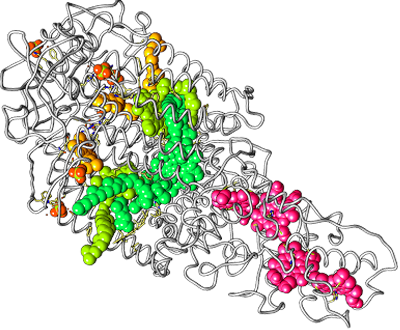
\includegraphics[scale=0.3]{protein.png}
				\end{minipage} 
			\end{center}
		}
		
		\headerbox{O Problema}{name=problem, column=0, below=intro}{
			Abordaremos aqui o problema de \textbf{encontrar as posições dos átomos de uma molécula}, tendo como entradas algumas distâncias entre átomos próximos (obtidas através de experimentos de Ressonância Magnética Nuclear \cite{crippen:DistancesAndMolecularConformation}). Este é conhecido na literatura como \textit{Molecular Distance Geometry Problem} (MDGP), que é uma particularização do \textit{Distance Geometry Problem} (DGP) \cite{carlileGDandAplications}. Tal problema, \textbf{munido de uma ordem conveniente} para percorrer seus átomos (dada pelo \textit{Discretization Vertex Order Problem}, ou simplesmente, DVOP), \textbf{pode ser discretizado}, gerando o \textit{Discretizable MDGP} (DMDGP), como segue formalmente definido \cite{carlile:MinimalOrder}.
		}
		
		\headerbox{DMDGP}{name=dmdgp, column=0, below=problem}{
			\textbf{Discretizable Molecular Distance Geometry Problem: }Dados um grafo ponderado e não-direcionado $G = (V,E,d)$, onde $d: E \longrightarrow \mathbb{R}_{+}$, o subconjunto de vértices iniciais $U_{0} = \{v_{1},v_{2},v_{3} \}$ e uma relação de ordem total em $V$ que satisfaz a seguinte relação de axiomas:
			\begin{enumerate}
				\vspace{-0.2cm}
				\item $G[U_{0}]$ é um clique em três vértices (iniciando a configuração);
				\vspace{-0.2cm}
				\item para todo vértice $v_{i}$ com posto $i = \rho(v_{i}) > 3$ nesta ordem, $G[U_{i}]$ é uma clique com quatro vértices (ordem de discretização, dada anteriormente) e
				\vspace{-0.2cm}
				\item para cada vértice $v_{i}$, com posto $i = \rho(v_{i}) > 3$, juntamente com $\{ v_{i-3}, v_{i-2} , v_{i-1} \}$, vale a desigualdade
				\vspace{-0.25cm}
				\begin{center}
					$d_{i-3,i-1} < d_{i-3,i-2} + d_{i-2,i-1},$ \hspace{0.5cm} (Desigualdade Triangular Estrita)
				\end{center}
			\end{enumerate}
			\vspace{-0.2cm}
			\underline{encontre uma imersão} $x: V \longrightarrow \mathbb{R}^{3}$ tal que valha $\left\| x(v_{i}) - x(v_{j}) \right\| = d_{i,j}$, $\forall \{v_{i},v_{j} \} \in E$.
		}
		
		\headerbox{Geometria das Proteínas}{name=geometria, column=0, below=dmdgp}{
			Para ser possível encontrar a ordem acima, precisamos estudar a geometria molecular. Felizmente existe uma \textit{subestrutura periódica} nas proteínas chamada \textbf{Cadeia Principal}, que possui uma geometria rica e bem conhecida \cite{bioquimicaLehninger}.
		}
		
		\headerbox{Cadeia Principal}{name=cadeia, column=1}{
			Através de dados experimentais de cristalografia, \textbf{sabe-se muito sobre a geometria média dessa subestrutura} \cite{ramachandran1974MolStructure} (também conhecida como \textit{backbone}, mostrada abaixo) onde \textbf{os comprimentos e ângulos} entre  as ligações dos átomos que a formam \textbf{são fixos}, na média, a menos de erros de medida. 
			
			\vspace{-0.25cm}
			\begin{center}
				\begin{minipage}{0.532\linewidth}
					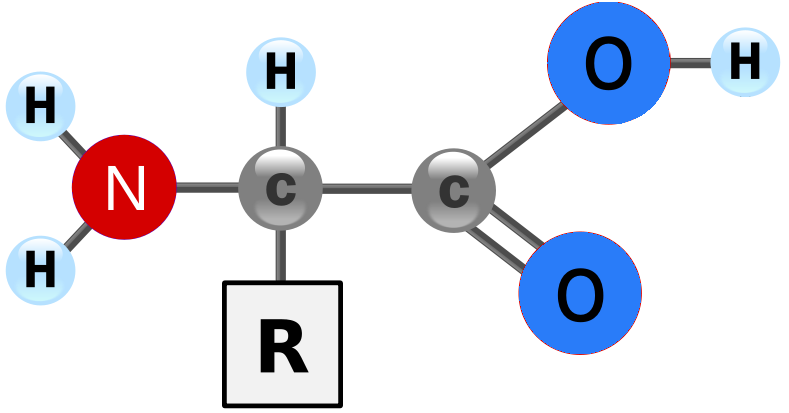
\includegraphics[scale=0.2]{amino.png}
				\end{minipage} 
			\end{center}
		}
		
		\headerbox{Ordem Conveniente}{name=order, column=1, below=cadeia}{
			Tendo posse dessas informações sobre a cadeia principal, pode-se pensar em percorrer os átomos da molécula \textbf{utilizando esta subestrutura como guia}, \textit{repetindo} os átomos que possuem propriedades conhecidas, afim de fazer valer os três axiomas do DMDGP. Isto foi feito em \cite{carlile:MinimalOrder} propondo o \textbf{\textit{hand-crafted vertex order}}, conforme esboça a figura abaixo (extraída do texto original). 
			
			\begin{minipage}{0.532\linewidth}
				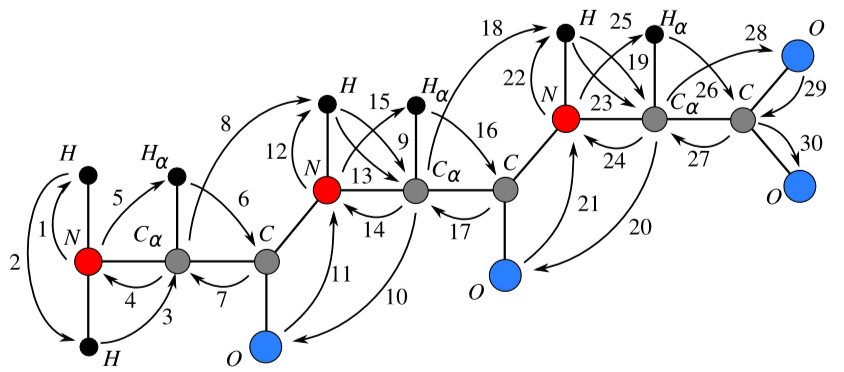
\includegraphics[scale=0.495]{hcVO.png}
				\vspace{-0.3cm}
			\end{minipage}
			
		}
		
		\headerbox{HC Order}{name=hc, column=1, below=order}{
			Seja $G = (V, E, d)$ o grafo associado a cadeia principal de uma proteína ($\{N^k, C^{k}_\alpha,C^k\}$, para $k = 1,\dots,p$), incluindo os átomos de oxigênio $O^k$, ligados ao $C^k$, e átomos de hidrogênio $H^k$ e $H^{k}_\alpha$, ligados ao $N^k$ e $C^{k}_\alpha$, respectivamente (conforme imagem acima, onde $p = 3$).
			
			Define-se a ordem HC como:
			
			\begin{small}
				\begin{minipage}{0.532\linewidth}
					$$
					hc = \{ N^1, H^1, H^{1'}, C_{\alpha}^1, N^1, H_{\alpha}^1, C^1, C_{\alpha}^1, \dots,
					$$
						
				\end{minipage}
				\vspace{-0.1cm}
				$$
				H^i, C_{\alpha}^i, O^{i-1}, N^i, H^i, C^{i}_\alpha, N^i, H^{i}_\alpha, C^i, C_{\alpha}^i,\dots,
				$$
				
				\hspace{.8cm}
				\begin{minipage}{0.532\linewidth}
					\vspace{-0.5cm}
					$$
					H^p, C_{\alpha}^p, O^{p-1}, N^p, H^p, C^{p}_\alpha, N^p,
					$$
					\vspace{-0.cm}
					\hspace{1.5cm}
					\begin{minipage}{0.532\linewidth}
					\vspace{-01.cm}
						$$
						 H^{p}_\alpha, C^p, C_{\alpha}^p, O^p, C^p, O^{p'}\}
						$$
					\end{minipage}
				\end{minipage}
			\end{small}
		
			Onde, como na figura, $i = 2, \dots, p-1$, $H^{1'}$ é o segundo hidrogênio ligado ao $N^1$ e $O^{p'}$ é o segundo oxigênio ligado ao $C^p$.
		}
	
		\headerbox{PDBReader}{name=pdbreader, column=1, below=hc}{
		Para facilitar o estudo da geometria molecular e as simulações do problema, o principal autor deste documento implementou um software (chamado \textbf{PDBReader}) que aceita como entrada instâncias de proteínas do repositório wwPDB e tem como saída um arquivo descrevendo a proteína \textbf{com sua instância reordenada} (utilizando ordenação HC). Perceba que esta é uma \textit{automação da discretização do problema}.
		
		O software permite atualmente três opções de saída (XML, matriz para Matlab e JSON), além de uma interface gráfica para visualização de uma projeção 2D da proteína.
		
		}
	
		\headerbox{GUI PDBReader}{name=gui, column=2}{
			Segue interface gráfica (GUI) do software.
			
			\begin{minipage}{0.532\linewidth}
				\hspace{-0.5cm}
				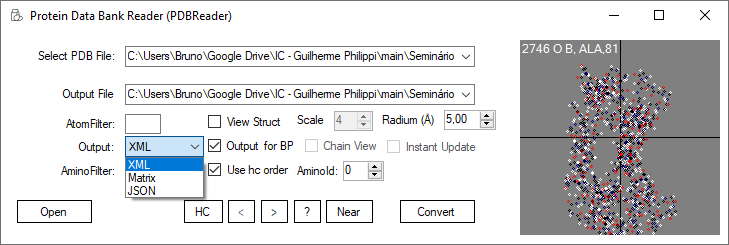
\includegraphics[scale=0.4]{output.png}
			\end{minipage}
		}
		
		\headerbox{Algorítimo Branch-\&-Prune }{name=conclusion, column=2,below=gui}{
			Ganhamos algumas vantagens com a discretização do problema pois a ordem no DMDGP garante a \textbf{finitude do conjunto solução} do problema e, além disso, organiza o espaço onde devemos fazer a busca por uma solução. Na verdade, a ordem induz uma estrutura de \textit{\textbf{árvore binária}} no espaço de busca \cite{fidalgotese}. De fato, sempre \textbf{temos duas possibilidades para posicionar o ângulo de torção} para o próximo átomo da molécula \cite{carlileGDandAplications}. Devido a esta estrutura, criou-se o algorítimo \textit{\textbf{Branch-\&-Prune}} (BP), que consiste em uma estratégia numérica \textit{recursiva} que resolve o DMDGP eficientemente utilizando uma busca combinatória no espaço de busca de soluções, onde realiza-se vértice por vértice do sistema, seguindo a ordem dada, ``podando'' todo sub-conjunto solução do sistema que não esteja de acordo com as informações pré-estabelecidas. 
			\begin{minipage}{1\linewidth}  
				\begin{minipage}{1.46\linewidth}  
					\vspace{.1cm}
					\hspace{4.2cm}
					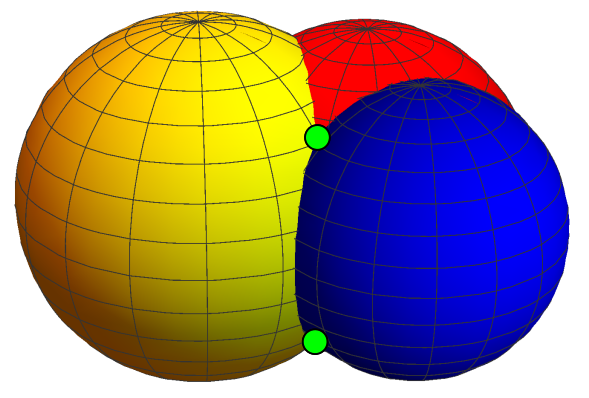
\includegraphics[scale=0.2]{dual.png}
				\end{minipage}
				\begin{minipage}{0.532\linewidth}
					\vspace{-2.2cm}
					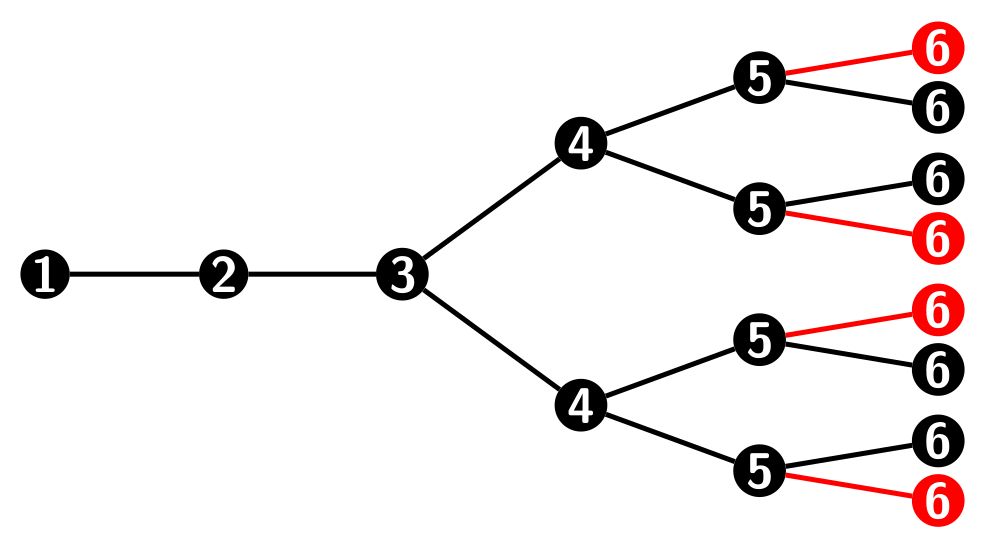
\includegraphics[scale=0.16]{bp.png}
				\end{minipage}
			\end{minipage}
		\vspace{-.2cm}
		
		}
		
		%\headerbox{Sponsors}{name=sponsor, column=2, above=bottom}{
		%\begin{center}
		% \includegraphics[scale=.5]{fapesp.jpg} \hspace*{.5cm} 
\includegraphics[scale=1]{cnpq.jpg} 
		%\end{center}
		%}
		
		\headerbox{Referências}{name=bibref, column=2, below=conclusion}{
			
			\renewcommand\refname{}
			% \renewcommand\bibname{}
			
			\bibliographystyle{ieee}
			\vspace{-0.6cm}
			\begin{thebibliography}{3}
				\begin{small}
					\bibitem{bioquimicaLehninger}
					David~L Nelson and Michael~M Cox.
					\newblock {\em Lehninger: principios de bioqu{\'\i}mica}.
					\newblock 2015.
					\vspace{-0.3cm}
					
					\bibitem{carlileBook31Coloquio}
					C.~Lavor, N.~Maculan, M.~Souza, and R.~Alves.
					\newblock {\em Álgebra e Geometria no Cálculo de Estrutura Molecular}.
					\newblock IMPA, Rio de Janeiro, RJ, 31º colóquio brasileiro de matemática
					edition, 2017.
					\vspace{-0.3cm}
					
					\bibitem{crippen:DistancesAndMolecularConformation}
					Gordon~M Crippen, Timothy~F Havel, et~al.
					\newblock {\em Distance geometry and molecular conformation}, volume~74.
					\newblock Research Studies Press Taunton, 1988.
					
					\vspace{-0.3cm}
					\bibitem{carlileGDandAplications}
					Leo Liberti, Carlile Lavor, Nelson Maculan, and Antonio Mucherino.
					\newblock Euclidean distance geometry and applications.
					\newblock {\em Society for Industrial and Applied Mathematics}, 56(1):3-69,
					February 2014.
					
					\vspace{-0.3cm}
					\bibitem{carlile:MinimalOrder}
					Carlile Lavor, Leo Liberti, Bruce Donald, Bradley Worley, Benjamin Bardiaux,
					Th{\'e}r{\`e}se~E Malliavin, and Michael Nilges.
					\newblock Minimal nmr distance information for rigidity of protein graphs.
					\newblock {\em Discrete Applied Mathematics}, 256:91--104, 2019.
					
					\vspace{-0.3cm}
					\bibitem{ramachandran1974MolStructure}
					GN~Ramachandran, AS~Kolaskar, C~Ramakrishnan, and V~Sasisekharan.
					\newblock The mean geometry of the peptide unit from crystal structure data.
					\newblock {\em Biochimica et Biophysica Acta (BBA)-Protein Structure},
					359(2):298--302, 1974.
					
					\vspace{-0.3cm}
					\bibitem{fidalgotese}
					Felipe Delfini~Caetano Fidalgo.
					\newblock {\em Dividindo e conquistando com simetrias em geometria de
						distâncias}.
					\newblock PhD thesis, UNICAMP, Campinas, SP, Fevereiro 2015.
				\end{small}
				\vspace{-0.2cm}
		\end{thebibliography}}
		
		\headerbox{Agradecimentos}{name=acknoledge, column=2,below=bibref}{
			{\footnotesize
				O presente trabalho foi realizado com o apoio do Conselho Nacional de Desenvolvimento	Científico e Tecnológico – CNPq – Brasil. Agradeço a Família e ao Felipão.}
		}
		
	\end{poster}%
\end{document}
